% ====================================================================
% VİZE RAPOR ŞABLONU – Türk Masalları Derlemesi Web Sayfası
% --------------------------------------------------------------------
% DERLEME: Overleaf'te Menu > Compiler > XeLaTeX (pdfLaTeX de çalışır).
%
% KURALLAR (şablonu kullanmadan önce okuyun):
%  1. Bölüm başlıklarını SİLMEYİN ve sırasını DEĞİŞTİRMEYİN.
%  2. [KÖŞELİ PARANTEZ] içindeki ve gri renkli açıklama metinlerini
%     kendi bilgilerinizle değiştirin; açıklama metinlerini silin.
%  3. MEBİS'e YALNIZCA bu raporun PDF'ini yükleyin.
%     ZIP ve HTML dosyası YÜKLEMEYİN. Tüm kontroller GitHub'dan yapılır.
%  4. Kapaktaki GitHub ve YouTube bağlantıları doğru ve tıklanabilir
%     olmalıdır. Teslimden önce PDF'teki bağlantılara tıklayıp deneyin.
%  5. Haftalık katkı tablosundaki görseller için resim dosyalarını
%     (hafta1.png, hafta2.png, ...) Overleaf projesine yükleyin.
%     Dosya adlarında boşluk ve Türkçe karakter kullanmayın.
%     Resim yoksa tabloda "görsel ekleyin" kutusu görünür.
%  6. Yapay zekâ kullandıysanız Bölüm 5'i doldurun.
% ====================================================================
\documentclass[12pt,a4paper]{article}

\usepackage{iftex}
\ifPDFTeX
  \usepackage[T1]{fontenc}
  \usepackage[utf8]{inputenc}
\else
  \usepackage{fontspec}
\fi
\usepackage[turkish]{babel}
\usepackage[margin=2.4cm]{geometry}
\usepackage{setspace}
\usepackage{graphicx}
\usepackage{booktabs}
\usepackage{longtable}
\usepackage{array}
\usepackage{colortbl}
\usepackage{xcolor}
\usepackage{enumitem}
\usepackage{listings}
\usepackage{amssymb}
\usepackage{caption}
\usepackage{fancyhdr}
\usepackage{hyperref}
\usepackage{float}
\usepackage{microtype}

\onehalfspacing
\setlength{\parindent}{0pt}
\setlength{\parskip}{6pt}
\setlist{itemsep=2pt, topsep=4pt}
\hypersetup{colorlinks=true, linkcolor=blue!50!black, urlcolor=blue!50!black}

\definecolor{ana}{HTML}{14325C}
\definecolor{acik}{HTML}{EEF2F8}

\lstset{basicstyle=\ttfamily\small, backgroundcolor=\color{acik},
  frame=single, rulecolor=\color{ana}, breaklines=true,
  columns=fullflexible, keepspaces=true, showstringspaces=false}

\pagestyle{fancy}
\fancyhf{}
\fancyhead[L]{MASALTI — Bir Kapı, On Masal}
\fancyhead[R]{Vize Raporu}
\fancyfoot[C]{\thepage}

% ---------- Yardımcı komutlar ----------
% Gri açıklama metni (silinecek yönergeler için)
\newcommand{\aciklama}[1]{{\color{gray}\itshape (#1)}}

% Haftalık tablo görseli: dosya yoksa "görsel ekleyin" kutusu çıkar
\newcommand{\haftagorsel}[1]{%
  \IfFileExists{#1}{%
    \includegraphics[width=\linewidth,height=4.2cm,keepaspectratio]{#1}%
  }{%
    \fbox{\parbox[c][2.6cm][c]{\dimexpr\linewidth-2\fboxsep-2\fboxrule\relax}{%
      \centering\small\color{gray} Ekran görüntüsü / görsel ekleyin\\ \texttt{#1}}}%
  }%
}
% Haftalık katılım kutuları (işaretlemek için $\square$ yerine $\boxtimes$ yazın)
\newcommand{\katilimkutulari}{\par\vspace{3pt}\small $\square$ Ders içinde katılım sergiledim\par $\square$ Telafi yaptım}

% Ek görsel: dosya yoksa hiçbir şey göstermez
\newcommand{\haftaek}[1]{%
  \IfFileExists{#1}{\\[4pt]\includegraphics[width=\linewidth,height=4.2cm,keepaspectratio]{#1}}{}%
}

% ---------- Kapak bilgileri ----------
\newcommand{\universite}{İstanbul Medipol Üniversitesi / Görsel İletişim Tasarımı}
\newcommand{\dersadi}{Programlamaya Giriş}
\newcommand{\hocaadi}{Meral Şentürk}
\newcommand{\ogrenciadi}{Ekrem Gökgez}
\newcommand{\ogrencino}{86230045}
\newcommand{\projeadi}{MASALTI: Bir Kapı, On Masal}
% Bağlantıları tam adres olarak yazın (https:// ile başlayarak)
\newcommand{\githublink}{\url{https://github.com/kseisi26-dotcom/Masalti}}
\newcommand{\youtubelink}{\textit{Bağlantı bekleniyor (video yükleme aşamasında).}}


\begin{document}
\shorthandoff{=}
\begin{titlepage}
\centering
\vspace*{1cm}
{\large \universite \par}
\vspace{1.8cm}
{\Huge\bfseries\color{ana} \projeadi \par}
\vspace{0.4cm}
{\Large Türk Masalları Derlemesi Web Sayfası \par}
{\large Vize Raporu \par}
\vspace{1.8cm}
{\large \textbf{Ders:} \dersadi \par}
{\large \textbf{Öğretim Üyesi:} \hocaadi \par}
\vspace{1.2cm}
{\large \textbf{Hazırlayan:} \ogrenciadi \par}
{\large \textbf{Öğrenci No:} \ogrencino \par}
\vspace{1.8cm}
\fbox{\parbox{0.88\linewidth}{\centering\vspace{6pt}
{\large\bfseries Proje Bağlantıları}\\[8pt]
\textbf{GitHub deposu:}\\ \githublink \\[8pt]
\textbf{YouTube sunum videosu:}\\ \youtubelink
\vspace{6pt}}}
\vfill
{\large 6 Kasım 2026 \par}
\end{titlepage}
\tableofcontents
\newpage

\section{Giriş}
MASALTI, Türk halk masallarını on farklı hikâye üzerinden daha görsel ve etkileşimli bir biçimde sunmak için hazırladığım web sitesi projesidir. Projenin çıkış noktası, masalları yalnızca art arda sıralanmış yazılar olarak göstermek yerine, her birine resimli bir okuma alanı hazırlamaktı. ``Bir varmış. Bir de sen.'' sloganı bu yaklaşımı özetliyor. Seçtiğim 10 masalı dörder resimli sahneye ayırdım; böylece toplam 40 hikâye sahnesi ortaya çıktı. Çalışmayı tek HTML dosyası, dosya içindeki CSS ve JavaScript kodlarıyla geliştirdim. Raporda masalların seçimini, arayüz tasarımını, kodun temel çalışma mantığını, yapay zekâ desteğini, ders çalışmalarını ve yapılan testleri anlatıyorum.

\subsection{Proje Özeti}
MASALTI'nın ana ekranında büyük bir karşılama illüstrasyonu ve masallar arasında sağ-sol geçiş yapılabilen bir alan bulunur. ``Masal Sandığı'' bölümünde on masal kart hâlinde sıralanır. Kullanıcı başlık ve açıklamaya göre arama yapabilir, okuduğu veya kaydettiği masalları filtreleyebilir ve rastgele bir masal seçebilir. Okuma sayfalarında dört resimli sahne, metinler, kaynak notu, yazı boyutu araçları ve gece modu yer alır. Kaydetme ve okundu durumları \texttt{localStorage} üzerinde tutulur. Masalların metinleri dosyanın içinde bulunduğu için temel okuma işlevi çevrimdışı da kullanılabilir; kaynak sitelerine gitmek ise internet gerektirir.

\subsection{Gereksinimlerin Karşılanması}
\begin{center}
\rowcolors{2}{acik}{white}
\begin{tabular}{@{}p{10.1cm}c@{}}
\toprule
\rowcolor{ana}\textcolor{white}{\textbf{Gereksinim}} & \textcolor{white}{\textbf{Durum}} \\
\midrule
Masal sayısı 8--12 arasında (10 masal) & $\boxtimes$ \\
Tek HTML dosyası & $\boxtimes$ \\
Stil kodları içsel (\texttt{style} etiketi içinde) & $\boxtimes$ \\
Betik kodları içsel (\texttt{script} etiketi içinde) & $\boxtimes$ \\
İçerikler çevrimdışı okunabilecek biçimde dosya içinde & $\boxtimes$ \\
JavaScript sayfada anlamlı işlevler görüyor & $\boxtimes$ \\
Masal metinleri kaynaklardan kısa biçimde yeniden uyarlandı & $\boxtimes$ \\
Mobil ekranlara uyumlu sayfa düzeni & $\boxtimes$ \\
\bottomrule
\end{tabular}
\end{center}
\textbf{Metinlere ilişkin açıklama:} Masal metinleri özgün kaynakların bire bir kopyası değildir; kaynak anlatılardan hareketle, yapay zekâ desteği de kullanılarak kısa uyarlamalar hazırlanmıştır. Bu nokta Bölüm 5'te ayrıca belirtilmiştir.

\section{Masalların Seçimi}
Masalları seçerken tek bir tür veya karaktere yoğunlaşmak istemedim. Zekâ, yardımlaşma, cesaret, sevgi, aile ilişkileri ve olağanüstü olaylar gibi farklı konuların koleksiyonda bulunmasına dikkat ettim. Böylece kullanıcı bir masalı bitirdiğinde diğerinde yeni bir olay örgüsüyle karşılaşabiliyor. Metinlerin dayandığı kaynaklar her masalın ``Bu Masalın İzi'' bölümünde bağlantı ve kısa not olarak gösterilir.

{\small
\begin{longtable}{@{}cp{4.4cm}p{2.5cm}p{5.5cm}@{}}
\toprule
\textbf{No} & \textbf{Masal} & \textbf{Tema} & \textbf{Seçilme nedeni} \\
\midrule
\endfirsthead
\toprule \textbf{No} & \textbf{Masal} & \textbf{Tema} & \textbf{Seçilme nedeni} \\ \midrule
\endhead
1 & Ali Cengiz Oyunu & Zekâ / dönüşüm & Değişen kimlikler ve çözüm bulma çabası, görsel olarak hareketli bir anlatım sağlıyor. \\
2 & Balıkçının Oğlu & Macera & Yolculuk ve beklenmedik karşılaşmalarla farklı bir masal atmosferi sunuyor. \\
3 & Değirmenci ile Tilki & Kurnazlık & Tilki karakteri üzerinden akıl yürütme ve mizahı koleksiyona ekliyor. \\
4 & Dört Öğüt & Öğüt / karar & Verilen öğütler üzerinden kararların sonuçlarını ele alıyor. \\
5 & Kabak Gelin & Olağanüstülük & Alışılmadık karakteri ve masalsı dönüşüm fikriyle çeşitlilik sağlıyor. \\
6 & Keloğlan ile Yılan, Köpek, Kedi ve Balık & Yardımlaşma & Birden fazla hayvan karakterin yer aldığı, farklı sahnelere ayrılabilen bir hikâye. \\
7 & Keloğlan ve Altın Bülbül & Macera / cesaret & Keloğlan figürünü başka bir olay örgüsüyle göstermeye olanak veriyor. \\
8 & Korkak Adam ve Devler & Korku / cesaret & Korku ve beklenmedik tepkileri içeren güçlü görsel sahnelere sahip. \\
9 & Tuz Kadar Sevgi & Sevgi / değer & Sevginin ifade edilme biçimi üzerinden duygusal bir karşılık oluşturuyor. \\
10 & Üç Turunçlar & Fantastik macera & Olağanüstü öğeleri ve olaylar arasındaki geçişleriyle koleksiyonu tamamlıyor. \\
\bottomrule
\end{longtable}}

\section{Tasarım Kararları}
MASALTI'nın tasarımını hazır bir site teması üzerinde kurmadım. Eski masal kitapları, baskı dokuları ve resimli hikâye sayfalarıyla ilişkili bir görsel anlayış oluşturmaya çalıştım. Bunun yanında sayfanın güncel bir web sitesi gibi kolay gezilebilir olmasına önem verdim.

\subsection{Konuya Uygunluk}
İlk ekranda tipografi ve illüstrasyon birlikte kullanılıyor. ``Bir varmış. Bir de sen.'' başlığı ve yanındaki çizim, kullanıcıya henüz masal seçmeden projenin atmosferini tanıtıyor. Masal kartları bir kitap koleksiyonu gibi düzenlendi. Her masalın kendine ait resmi, kısa açıklaması ve okuma bağlantısı var. Okuma ekranında ise metnin yanında büyük görsellere yer verildi; böylece illüstrasyon yalnızca süs olarak kalmıyor, hikâyeyi takip etmeye yardımcı oluyor.

\subsection{Renk Paleti ve Yazı Tipi}
Renk kodları son HTML dosyasının \texttt{:root} tanımından alınmıştır.
\begin{center}
\rowcolors{2}{acik}{white}
\begin{tabular}{@{}p{3cm}p{2.5cm}p{7.7cm}@{}}
\toprule
\rowcolor{ana}\textcolor{white}{\textbf{Ad}} & \textcolor{white}{\textbf{Kod}} & \textcolor{white}{\textbf{Kullanım ve gerekçe}} \\
\midrule
Krem (kâğıt) & \texttt{\#F4EAD7} & Ana zemin; eski kitap sayfasını çağrıştıran açık ve sakin bir alan. \\
Koyu mürekkep & \texttt{\#24271F} & Başlık, metin, kontur ve butonlarda güçlü karşıtlık. \\
Kiremit kırmızısı & \texttt{\#C64C39} & Başlık vurguları ve ayırıcı grafik alanlar. \\
Koyu yeşil & \texttt{\#27796D} & Masal atmosferini güçlendiren tamamlayıcı renk. \\
Altın sarısı & \texttt{\#E6AD42} & Küçük vurgular ve dikkat çekmesi gereken kontroller. \\
Başlık / metin & -- & Büyük başlıklarda serif karakterler; arayüz ve yardımcı metinlerde sade sans-serif yapı. \\
\bottomrule
\end{tabular}
\end{center}

\subsection{Okunabilirlik, Gezinme ve Duyarlı Tasarım}
\begin{itemize}
\item \textbf{Okunabilirlik:} Başlıklar, açıklamalar ve masal metinleri için farklı büyüklükler kullandım. Okuma alanında satır aralıkları geniş; yazıyı büyütme/küçültme ve gece modu seçenekleri var.
\item \textbf{Gezinme:} Ana sayfadan masal kartlarına, arama alanına veya rastgele masal düğmesine geçilebiliyor. Kayıtlı ve okunmamış masalları ayrı filtrelemek mümkün.
\item \textbf{Duyarlı tasarım:} CSS Grid ve Flexbox ile oluşturulan alanlar \texttt{@media} kurallarıyla dar ekranlarda yeniden düzenleniyor. Görsel ve metinlerin yerleşimi telefon ekranında değişiyor.
\item \textbf{Tutarlılık:} Kart kenarlıkları, tipografik hiyerarşi, renk paleti ve illüstrasyon karakteri sayfa boyunca tekrar ediyor.
\end{itemize}

\subsection{Ekran Görüntüleri}
Aşağıdaki ekran görüntüleri MASALTI'nın masaüstü ve telefon görünümünden alınmıştır.
\begin{figure}[H]
\centering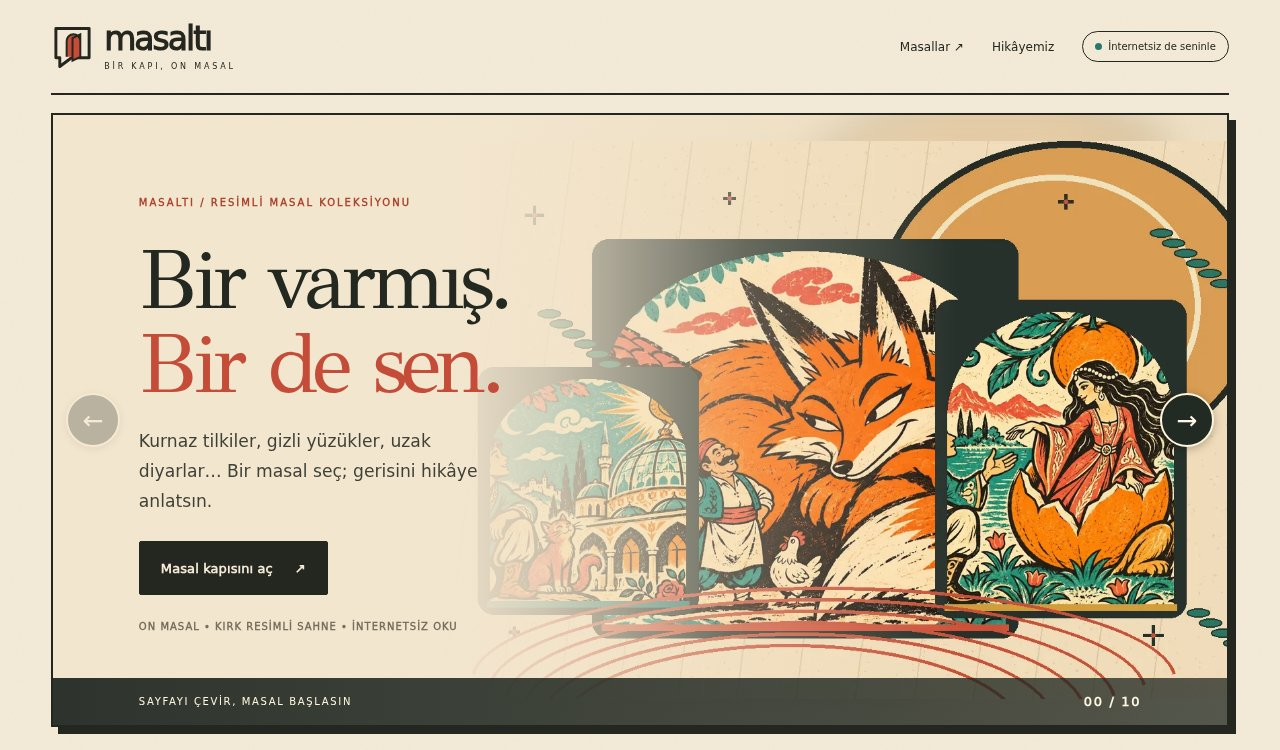
\includegraphics[width=.95\textwidth,height=8cm,keepaspectratio]{ekran-anasayfa.jpg}
\caption{MASALTI: ana sayfa, slogan ve karşılama illüstrasyonu.}
\end{figure}
\begin{figure}[H]
\centering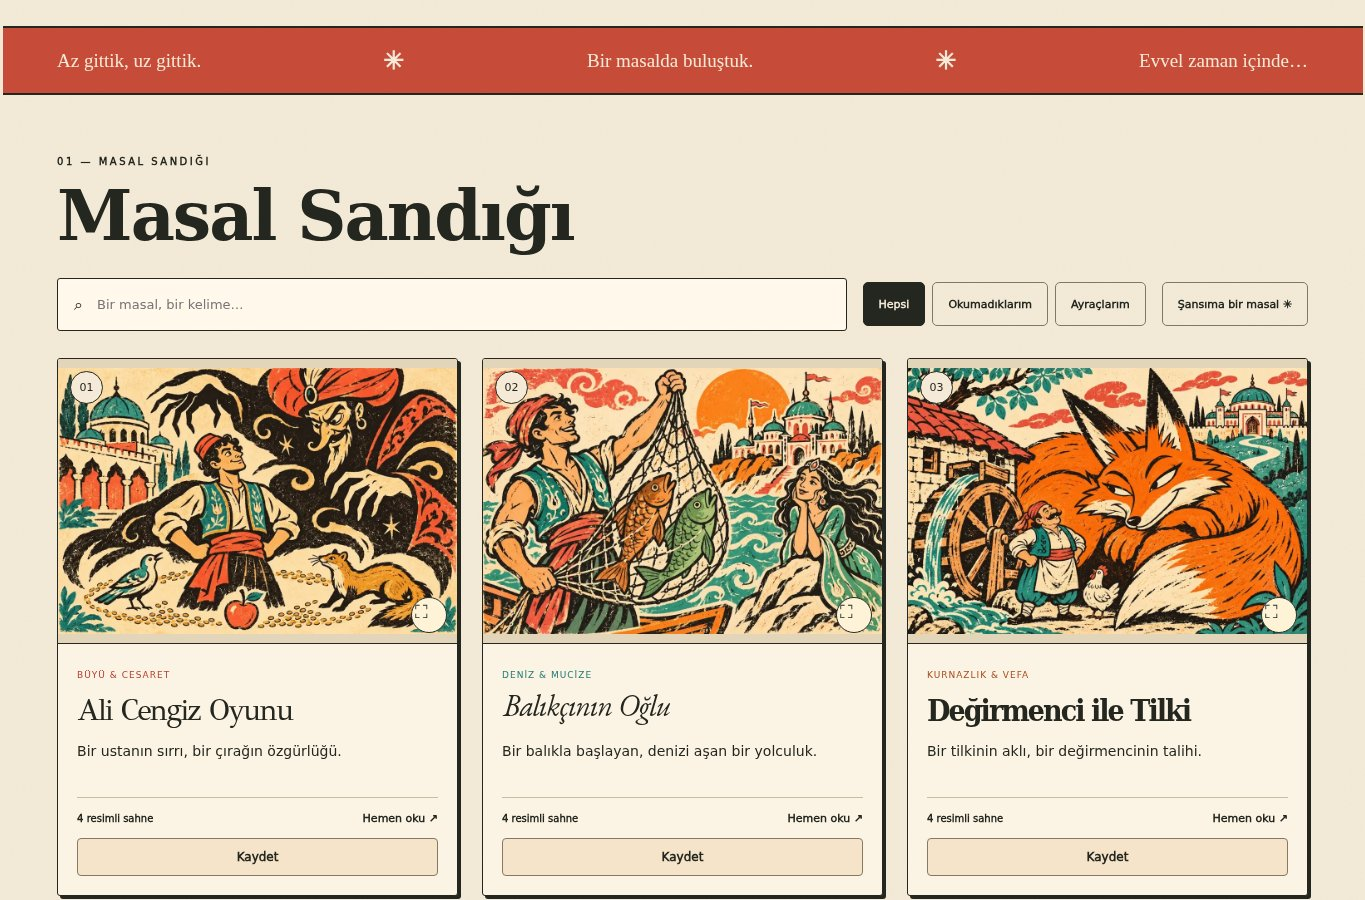
\includegraphics[width=.93\textwidth,height=7cm,keepaspectratio]{ekran-koleksiyon.jpg}
\caption{Masal Sandığı: arama, filtreleme ve resimli masal kartları.}
\end{figure}
\begin{figure}[H]
\centering
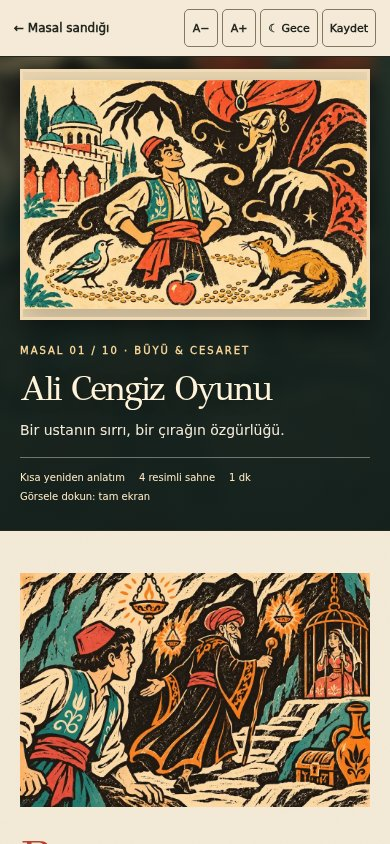
\includegraphics[height=9.1cm,keepaspectratio]{ekran-okuma.jpg}\hspace{1cm}
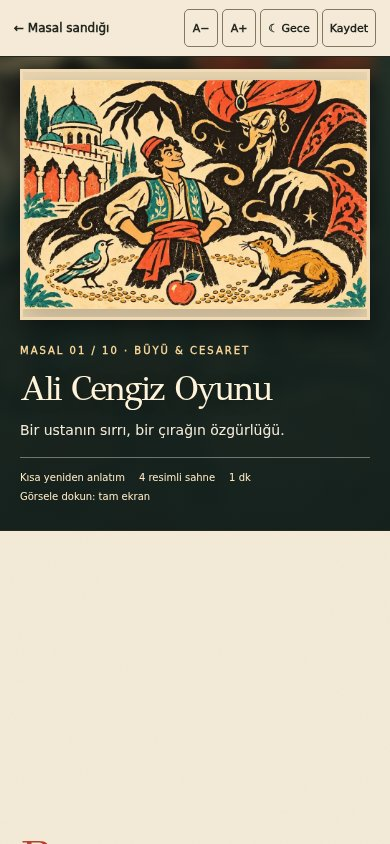
\includegraphics[height=9.1cm,keepaspectratio]{ekran-mobil.jpg}
\caption{Masal okuma ekranı ve dar ekran görünümünden örnekler.}
\end{figure}

\section{Gerçekleştirme}
Bu bölümde kullandığım temel kod yapılarını, tamamını kopyalamadan, anlaşılır kısa örneklerle açıklıyorum. Son sürümde görsel ve yazı tipi verileri de HTML'in içine gömüldüğü için dosya boyutu yaklaşık 15 MB'dır. Kod sunumunda işlevlerle ilgili kısa bölümlere odaklandım.

\subsection{HTML Yapısı}
Belge \texttt{<!DOCTYPE html>} ile başlıyor ve dil \texttt{lang="tr"} olarak tanımlanıyor. \texttt{head} içinde karakter kodlaması, ekran genişliği ve sayfanın açıklaması yer alıyor. \texttt{style} etiketiyle CSS aynı dosyada tutuluyor. \texttt{body} içinde karşılama alanı, Masal Sandığı, masal kartları, ayrı \texttt{article} okuma bölümleri ve sayfa sonu bilgileri bulunuyor. On masalın her birine \texttt{masal-0} ile \texttt{masal-9} arasında bir kimlik verildi. Böylece bağlantılarla ilgili hikâyeye geçilebiliyor. Masal metinleri ve görseller HTML içinde yer aldığından JavaScript devre dışı olsa bile temel metin erişimi korunacak şekilde bir düzen kuruldu.

\begin{lstlisting}[caption={HTML belgesinin baslangicindan kisa ornek}]
<!DOCTYPE html>
<html lang="tr">
<head>
  <meta charset="utf-8">
  <meta name="viewport" content="width=device-width,initial-scale=1">
</head>
\end{lstlisting}

\subsection{İçsel CSS}
CSS kodu HTML'in \texttt{style} alanında bulunuyor. \texttt{:root} ile tanımladığım renk değişkenlerini sayfanın farklı bölümlerinde kullandım. \texttt{display:grid} masal kartlarının sütun düzeninde, \texttt{display:flex} ise araç çubukları ve buton hizalamalarında yer alıyor. \texttt{@media(max-width:600px)} gibi kurallar telefon ekranlarında boşluk, yazı boyutu ve içerik akışını değiştiriyor.

\begin{lstlisting}[caption={Gercek dosyadaki renk degiskenleri ve kart duzeni}]
:root{
  --paper:#f4ead7;
  --ink:#24271f;
  --red:#c64c39;
  --teal:#27796d;
  --gold:#e6ad42;
}
.grid{display:grid;grid-template-columns:repeat(3,minmax(0,1fr));gap:24px}
@media(max-width:950px){.grid{grid-template-columns:repeat(2,minmax(0,1fr))}}
\end{lstlisting}

\subsection{İçsel JavaScript}
JavaScript kodları HTML'in \texttt{script} bölümünde yer alıyor. \texttt{norm()} arama metnini karşılaştırmaya uygun biçime getiriyor. \texttt{refresh()} arama ve seçili filtreye göre kartların görünürlüğünü değiştiriyor. \texttt{select(n)} ana sayfadaki seçili masalı, başlığı ve görseli güncelliyor. \texttt{route()} adresin sonundaki masal kimliğine göre ilgili okuma alanını açıyor. Kaydedilen ve okunan masallar \texttt{localStorage} ile tarayıcıda saklanıyor.

\begin{lstlisting}[caption={Arama ve filtre isleminin gercek JavaScript kodundan alinti}]
function refresh(){
  const q=norm(search.value);let count=0;
  cards.forEach((c,i)=>{
    const show=norm(c.dataset.search).includes(q)
      &&(filter!=='saved'||store.saved.includes(i))
      &&(filter!=='unread'||!store.read.includes(i));
    c.hidden=!show;
    if(show)count++;
  });
}
\end{lstlisting}

\begin{lstlisting}[caption={Tarayiciya kayit isleminin gercek koddan alintisi}]
function persist(){
  try{
    localStorage.setItem('masalti-v3',JSON.stringify(store));
    return true;
  }catch(e){return false}
}
\end{lstlisting}

\subsection{Sayfanın Özellikleri}
\begin{itemize}
\item \textbf{Masal keşfi:} Açılış bölümündeki oklarla masallar arasında geçiş; Masal Sandığı'nda on resimli kart.
\item \textbf{Arama ve filtreler:} Masalları arama, kaydedilenleri ve henüz okunmamış olanları ayrı gösterme.
\item \textbf{Rastgele seçim:} ``Şansıma Bir Masal'' düğmesiyle rastgele bir hikâyeye geçiş.
\item \textbf{Okuma araçları:} Yazı boyutunu değiştirme, gece modu ve görselleri daha büyük açma.
\item \textbf{Okuma takibi:} ``Bu Masalı Okudum'' işlemi ve okuma durumunun kartta görünmesi.
\item \textbf{Kayıt sistemi:} Okundu ve kaydedildi bilgilerinin tarayıcının yerel depolama alanında korunması.
\item \textbf{Tek dosya:} HTML, CSS, JavaScript ve görsellerin aynı dosyada bulunması.
\end{itemize}

\section{Yapay Zekâ Kullanımı}
Projede yapay zekâ desteğinden yararlandım. Özellikle masal anlatımlarını kaynaklardan hareketle kısaltma, resimli sahneleri üretme, HTML/CSS/JavaScript kodlarını geliştirme ve hata ayıklama aşamalarında ChatGPT desteği kullandım. Metinlerin yapay zekâ destekli kısa uyarlamalar olduğunu masal sayfalarındaki kaynak notlarında da belirttim. Tasarım kararlarını, arayüzün hangi özelliklere sahip olması gerektiğini ve revizyonların yönünü proje boyunca değerlendirdim.

{\small
\begin{longtable}{@{}p{2.3cm}p{3.8cm}p{4.6cm}p{3cm}@{}}
\toprule
\textbf{Araç} & \textbf{Kullanım amacı} & \textbf{İstem / yönlendirme özeti} & \textbf{Projede bulunduğu yer} \\
\midrule
\endhead
ChatGPT & Kodlama ve hata ayıklama & Tek HTML dosyası, mobil yerleşim, masal arama, filtreleme ve kaydetme işlevlerini geliştirme ve gözden geçirme. & HTML, CSS, JavaScript \\
ChatGPT destekli görsel üretimi & Masalları resimlendirme & Her masal için sahneye uygun, ortak karakter taşıyan resimli anlatım oluşturma. & Masal kapakları ve sahneleri \\
ChatGPT & Metinleri yeniden anlatma & Kaynak masalları doğrudan kopyalamadan kısa, dört bölümlü okuma metinlerine dönüştürme. & On masalın kısa uyarlamaları \\
ChatGPT & Rapor düzenleme & Kendi projemin ve paylaştığım ders kanıtlarının açıklamalarını resmî LaTeX şablonuna yerleştirme. & Bu rapor \\
\bottomrule
\end{longtable}}

\subsection{Anladığım ve Kendim Yaptığım Kısımlar}
Projenin adını, sloganını, eski masal kitabıyla modern arayüzü birleştirme fikrini, renk ve tipografi yönünü belirledim. İlk arayüz tasarımlarını ve farklı düzenleri değerlendirerek masal kartları, okuma alanı, başlık düzeni ve mobil görünüm üzerinde revizyonlar istedim. Kullanıcı açısından masal arama, kaydetme ve okunmuş olarak işaretleme gibi özelliklerin bulunmasını özellikle önemsedim. Kodlamada yapay zekâ desteğinden yararlandığım için bütün kodları sıfırdan ve tek başıma yazdığımı iddia etmiyorum. Bunun yerine HTML'in sayfa yapısını, CSS'in görsel düzeni ve JavaScript'in etkileşimleri nasıl yönettiğini öğrenmeye; işlevleri gerçek sayfada deneyerek kontrol etmeye çalıştım. GitHub Pages üzerinden telefon testi yapmam da bu sürecin bir parçası oldu.

\section{Haftalık Katkılar}
Aşağıdaki çalışmalar, ders kapsamında yaptığım ve ekran görüntülerini sakladığım uygulamalardır. Görseller üzerindeki tarihler dosya kaydıyla ilgilidir; bunları kesin ders tarihi gibi göstermiyorum. Birinci ve ikinci hafta aynı World Wide Web çalışmasının farklı kod ve önizleme bölümleriyle belgelenmiştir. Üçüncü haftada Moodify, dördüncü haftada bir renk bulmacası, beşinci haftada portfolyo uygulamaları ve altıncı haftada temel web / JavaScript örnekleri bulunmaktadır. Yedinci ve sekizinci haftaya ait ayrı bir etkinlik kanıtı paylaşılmadığı için çalışılmış gibi eklenmemiştir. Haftalık GitHub commit bağlantıları doğrulanamadığı için uydurulmamıştır.

{\footnotesize
\begin{longtable}{@{}>{\raggedright\arraybackslash}p{1.75cm}>{\raggedright\arraybackslash}p{6.4cm}>{\centering\arraybackslash}p{5.9cm}@{}}
\toprule
\rowcolor{ana}\textcolor{white}{\textbf{Hafta}} & \textcolor{white}{\textbf{Yapılan çalışma}} & \textcolor{white}{\textbf{Görsel kanıt}} \\
\midrule
\endfirsthead
\toprule
\rowcolor{ana}\textcolor{white}{\textbf{Hafta}} & \textcolor{white}{\textbf{Yapılan çalışma}} & \textcolor{white}{\textbf{Görsel kanıt}} \\
\midrule
\endhead
\bottomrule
\endfoot
\textbf{1. hafta}\newline Tarih: teyit edilmedi & World Wide Web konulu HTML sayfasında başlık, paragraf, sayfa iskeleti ve gezinme bağlantılarını denedim. Kod ile yan yana görünen önizlemenin nasıl değiştiğini karşılaştırdım.\newline \textbf{Commit:} Haftalık bağlantı doğrulanmadı.\newline Katılım/telafi bilgisi teyit edilmedi. & \haftagorsel{hafta1.jpg} \\
\midrule
\textbf{2. hafta}\newline Tarih: teyit edilmedi & Aynı World Wide Web çalışmasında içsel CSS ile lacivert zemin, turkuaz başlıklar, bölüm kutuları ve metin aralıklarını düzenledim. İçeriklerin hiyerarşisini ve sayfa içi gezinmeyi inceledim.\newline \textbf{Commit:} Haftalık bağlantı doğrulanmadı.\newline Katılım/telafi bilgisi teyit edilmedi. & \haftagorsel{hafta2.jpg} \\
\midrule
\textbf{3. hafta}\newline Tarih: teyit edilmedi & \textbf{Moodify:} Spotify'dan esinlenen koyu ve yeşil arayüzde demo giriş ekranı, dört ruh hâli kartı ve şarkı öneri alanı tasarladım. Ruh hâline göre önerilerin değişmesini JavaScript ile denedim.\newline \textbf{Commit:} Haftalık bağlantı doğrulanmadı.\newline Katılım/telafi bilgisi teyit edilmedi. & \haftagorsel{hafta3.jpg} \\
\midrule
\textbf{4. hafta}\newline Tarih: teyit edilmedi & \textbf{Dört Rengi Ayır:} Altı tüplü renk eşleştirme oyununda JavaScript ile tüp seçme, renk taşıma, hamle sayısını güncelleme ve kazanma ekranı hazırladım. Oyunu yeniden başlatma düğmesi de bulunuyor.\newline \textbf{Commit:} Haftalık bağlantı doğrulanmadı.\newline Katılım/telafi bilgisi teyit edilmedi. & \haftagorsel{hafta4.jpg} \\
\midrule
\textbf{5. hafta}\newline Tarih: teyit edilmedi & Kişisel portfolyom için önce temel HTML içerik düzenini (\texttt{task1.html}), ardından daha belirgin tipografi, gezinme ve boşluklara sahip ikinci bir tasarım görünümünü denedim.\newline \textbf{Commit:} Haftalık bağlantı doğrulanmadı.\newline Katılım/telafi bilgisi teyit edilmedi. & \haftagorsel{hafta5.jpg} \\
\midrule
\textbf{6. hafta}\newline Tarih: teyit edilmedi & Görsel İletişim Tasarımı konusunda bir bilgilendirme sayfası, JavaScript'te ışığı aç/kapat denemesi ve Bootstrap kart / grid düzeni kullanılan kapsamlı portfolyo uygulamasını hazırladım.\newline \textbf{Commit:} Haftalık bağlantı doğrulanmadı.\newline Katılım/telafi bilgisi teyit edilmedi. & \haftagorsel{hafta6.jpg} \\
\end{longtable}}

\textbf{Ek görsel kanıtlar:} Aşağıda üçüncü ve sonraki haftalardaki çalışmaların farklı durumları da gösterilmektedir.
\begin{figure}[H]\centering
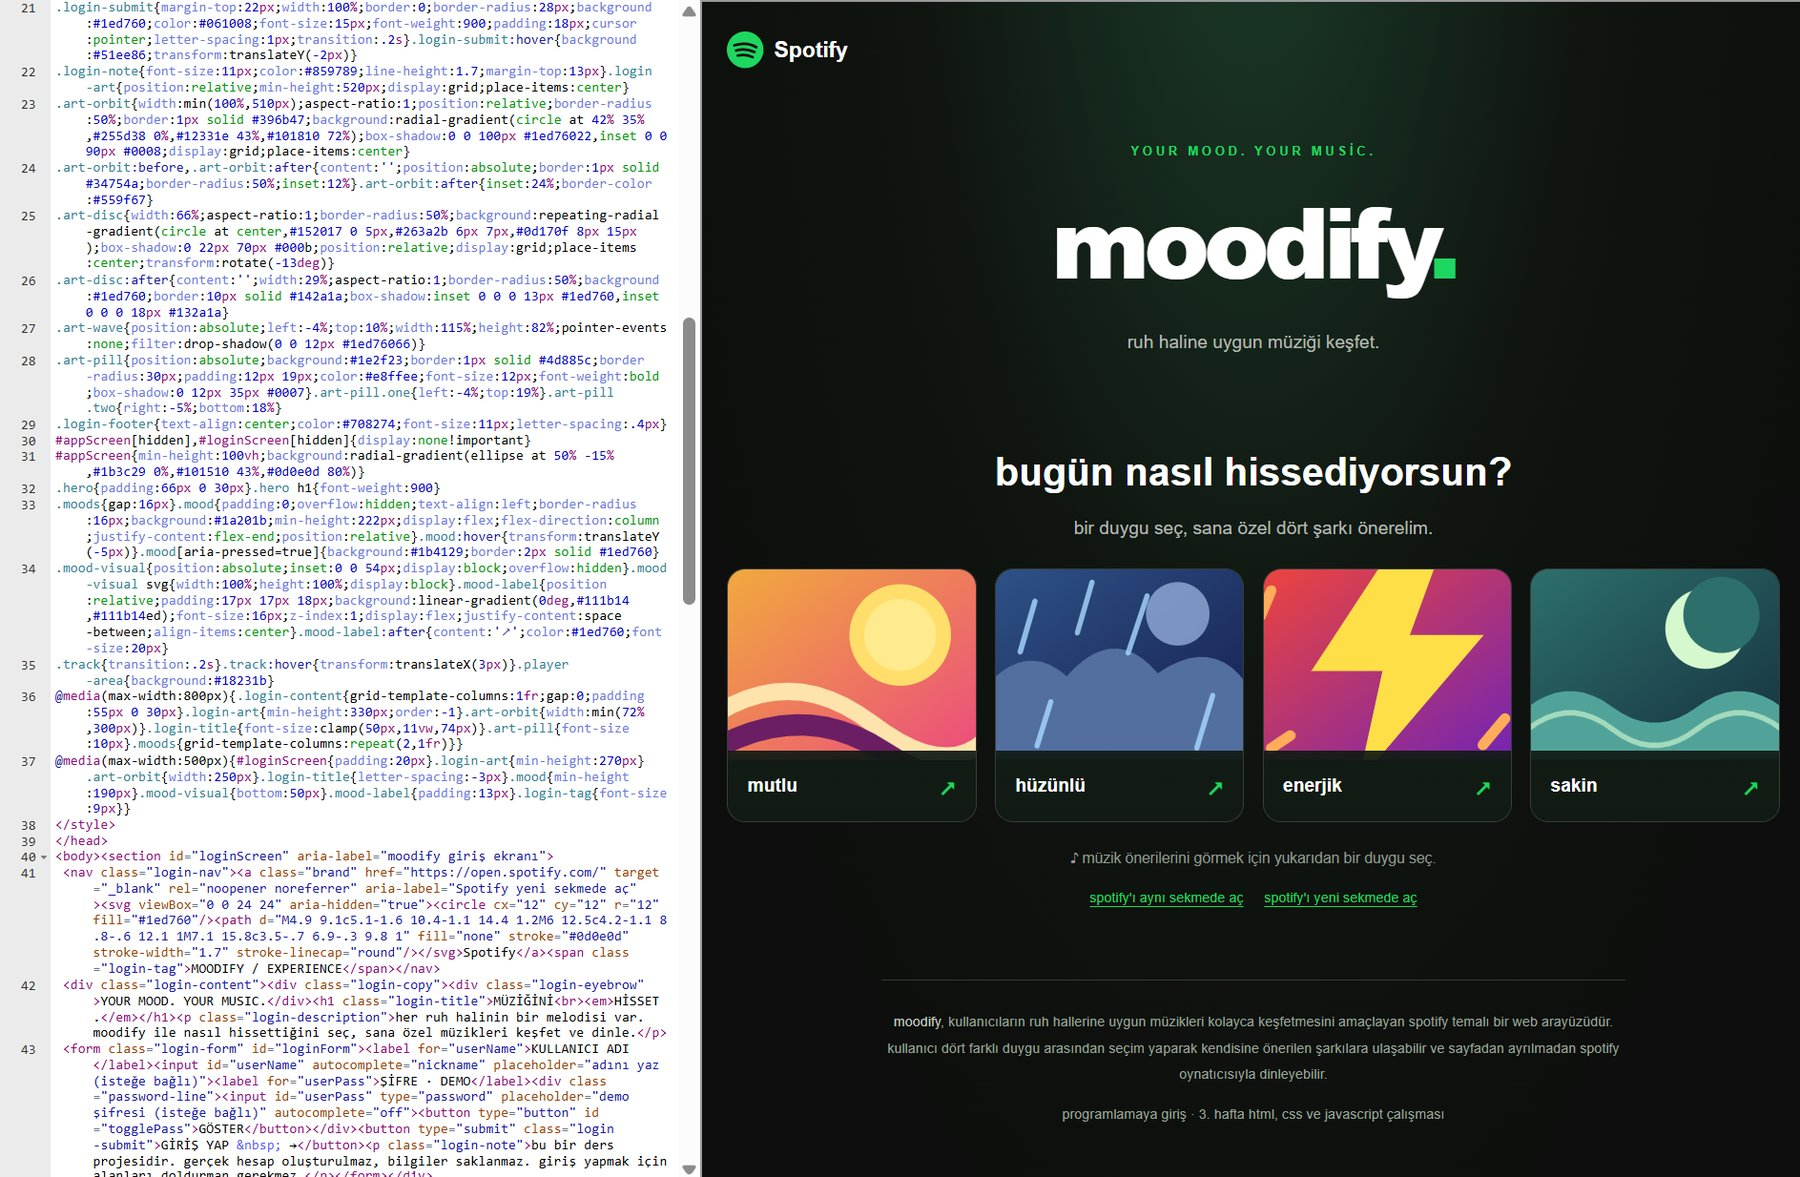
\includegraphics[width=.48\linewidth]{hafta3b.jpg}\hfill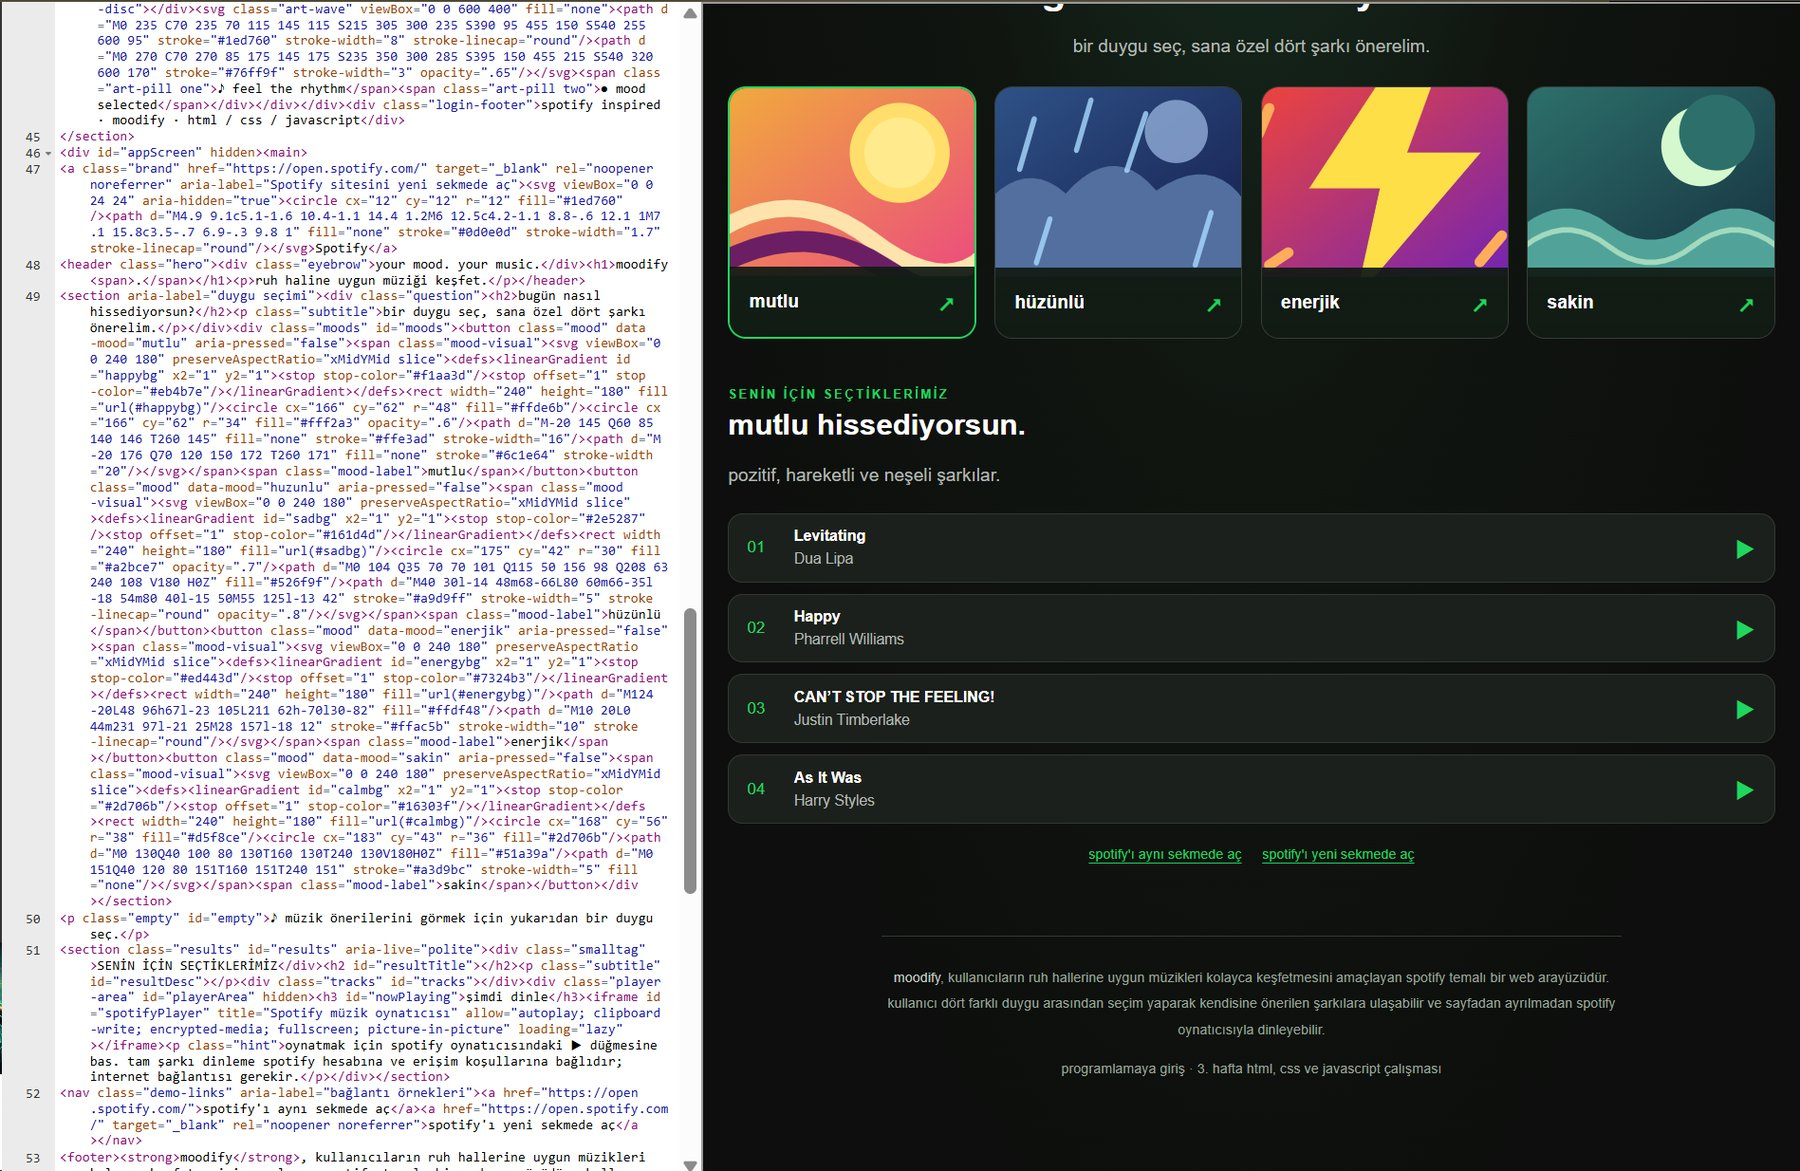
\includegraphics[width=.48\linewidth]{hafta3c.jpg}
\caption{3. hafta Moodify: ruh hâli kartları ve seçilen ruh hâline ait müzik önerileri.}
\end{figure}
\begin{figure}[H]\centering
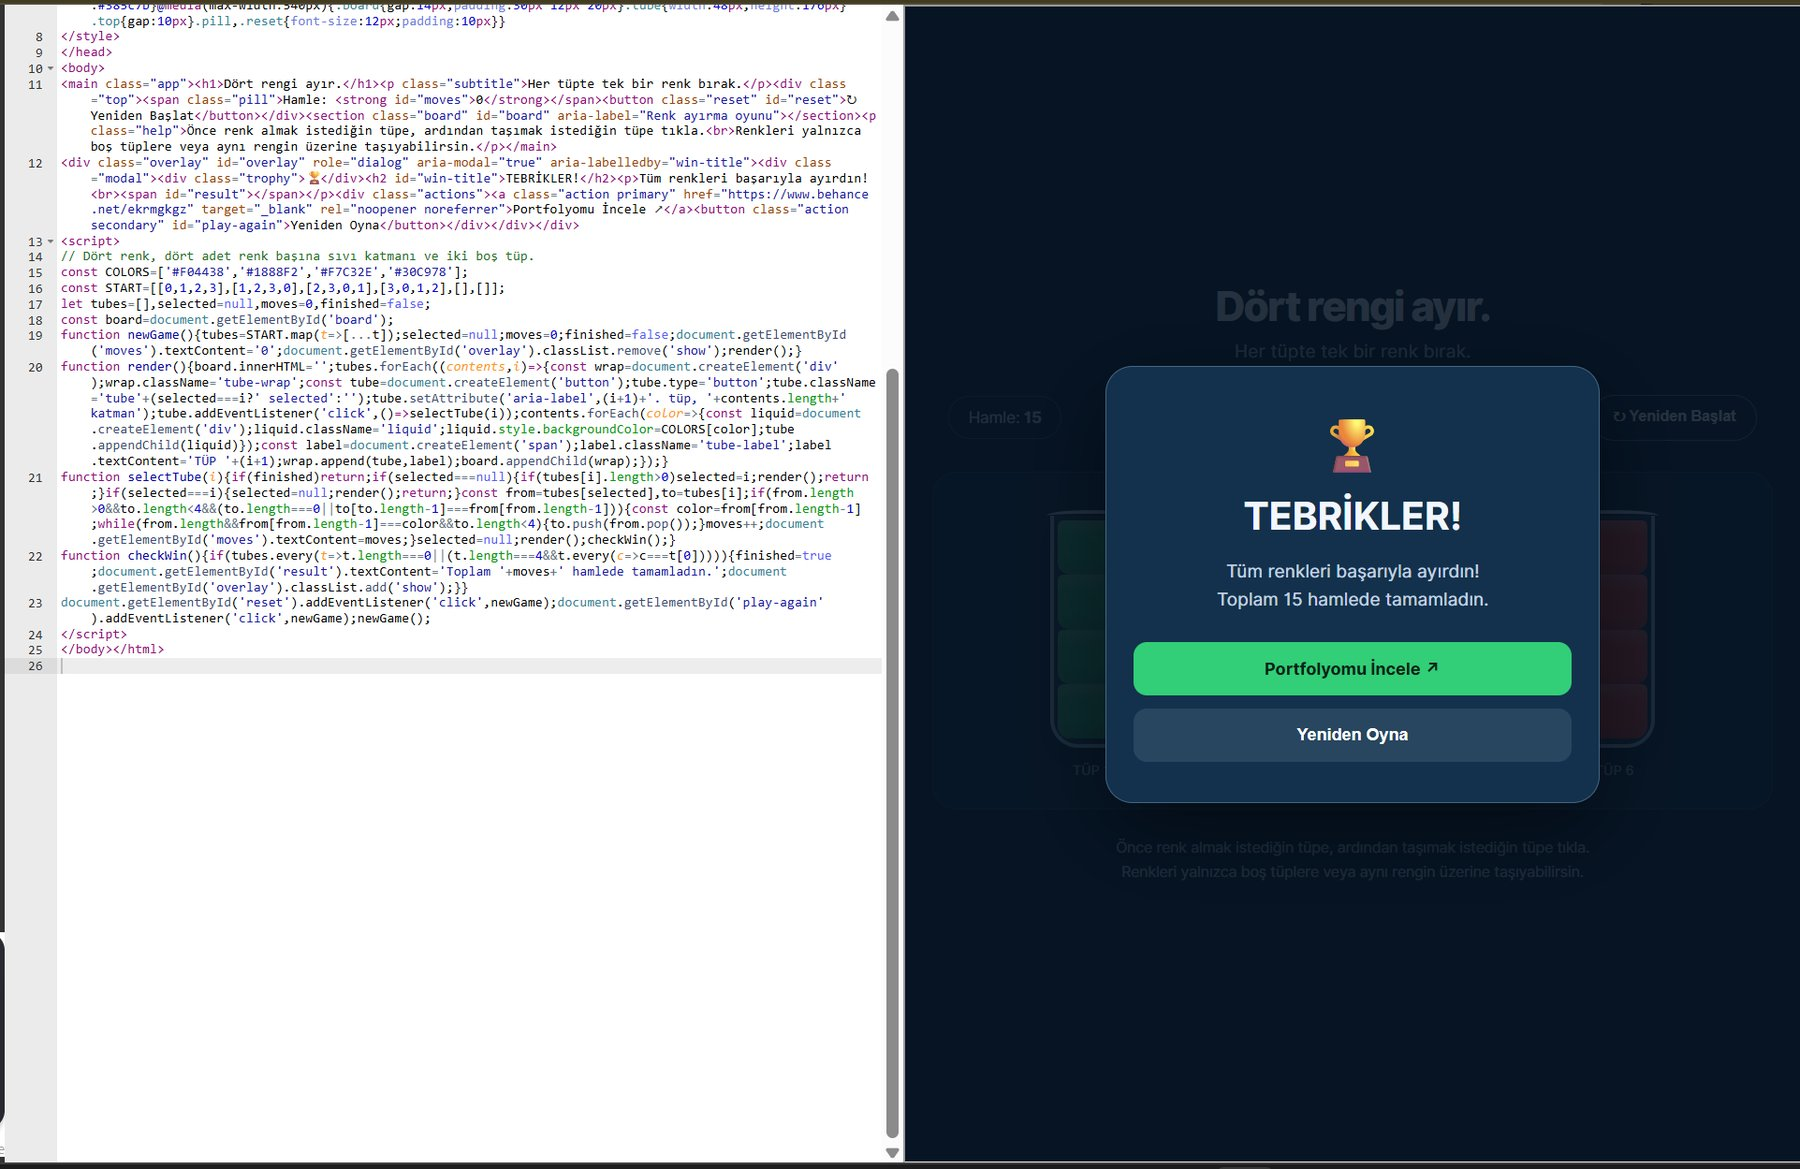
\includegraphics[width=.48\linewidth]{hafta4b.jpg}\hfill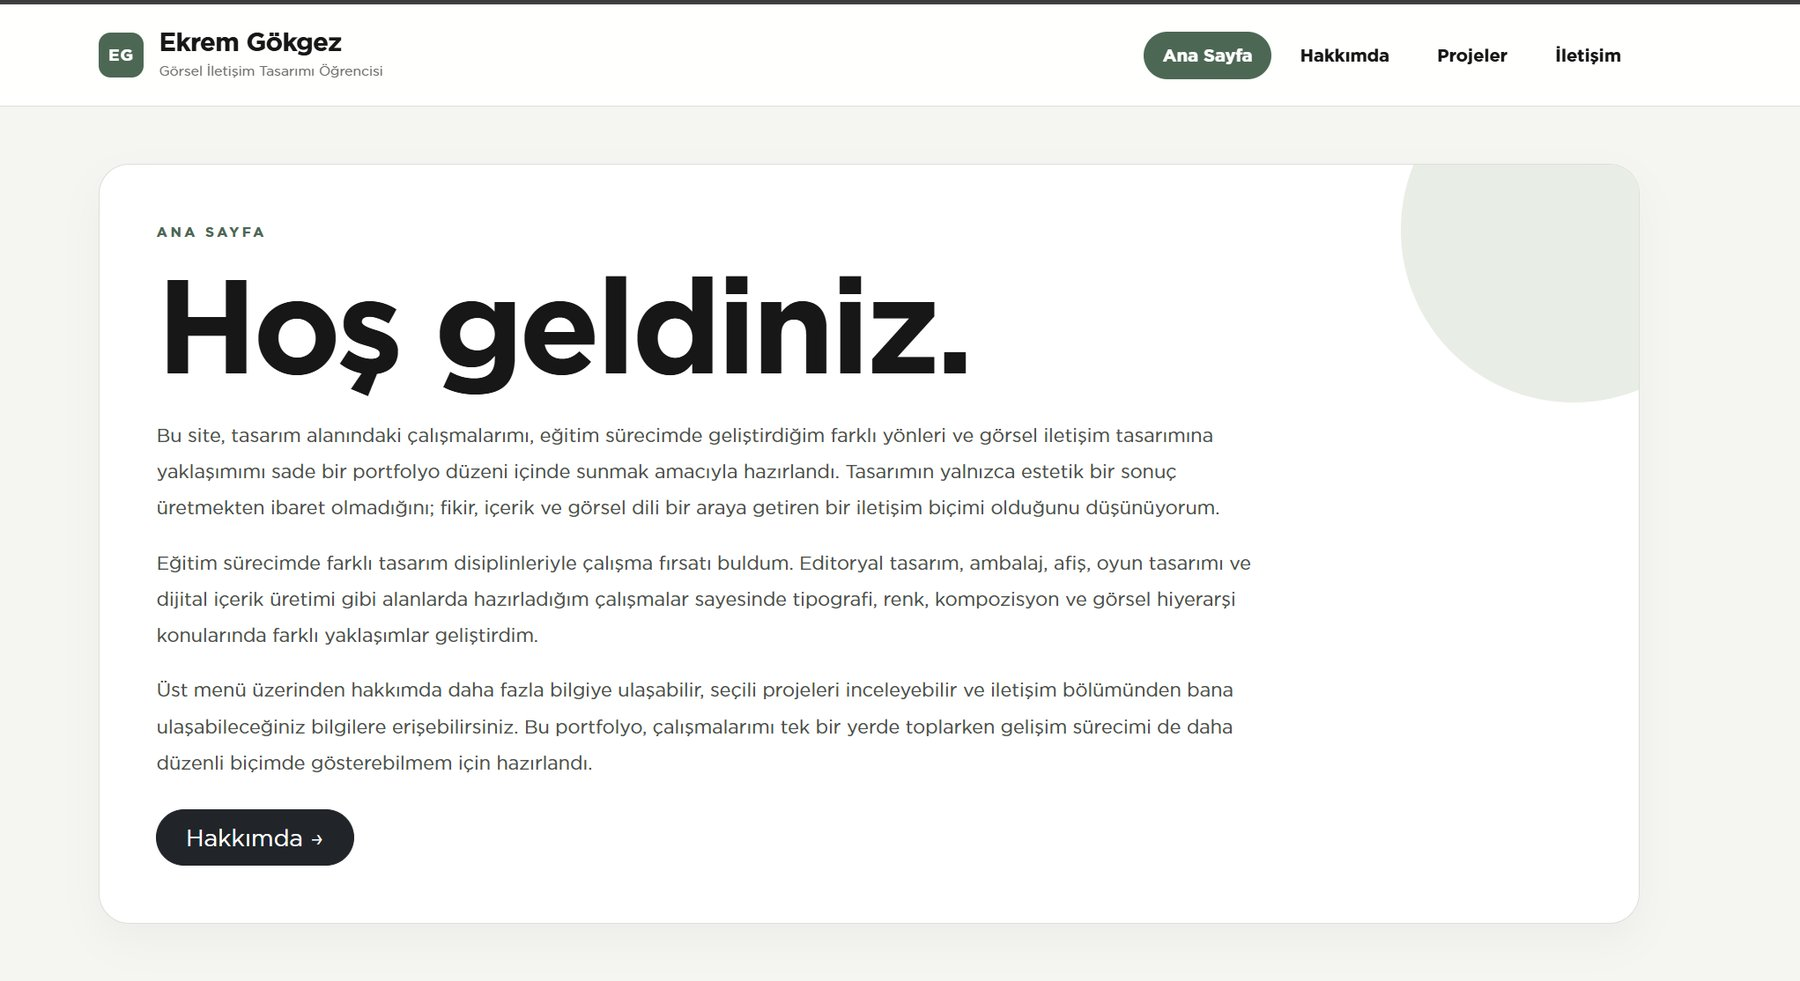
\includegraphics[width=.48\linewidth]{hafta5b.jpg}
\caption{4. hafta bulmaca oyununun bitiş ekranı; 5. hafta portfolyonun geliştirilmiş görünümü.}
\end{figure}
\begin{figure}[H]\centering
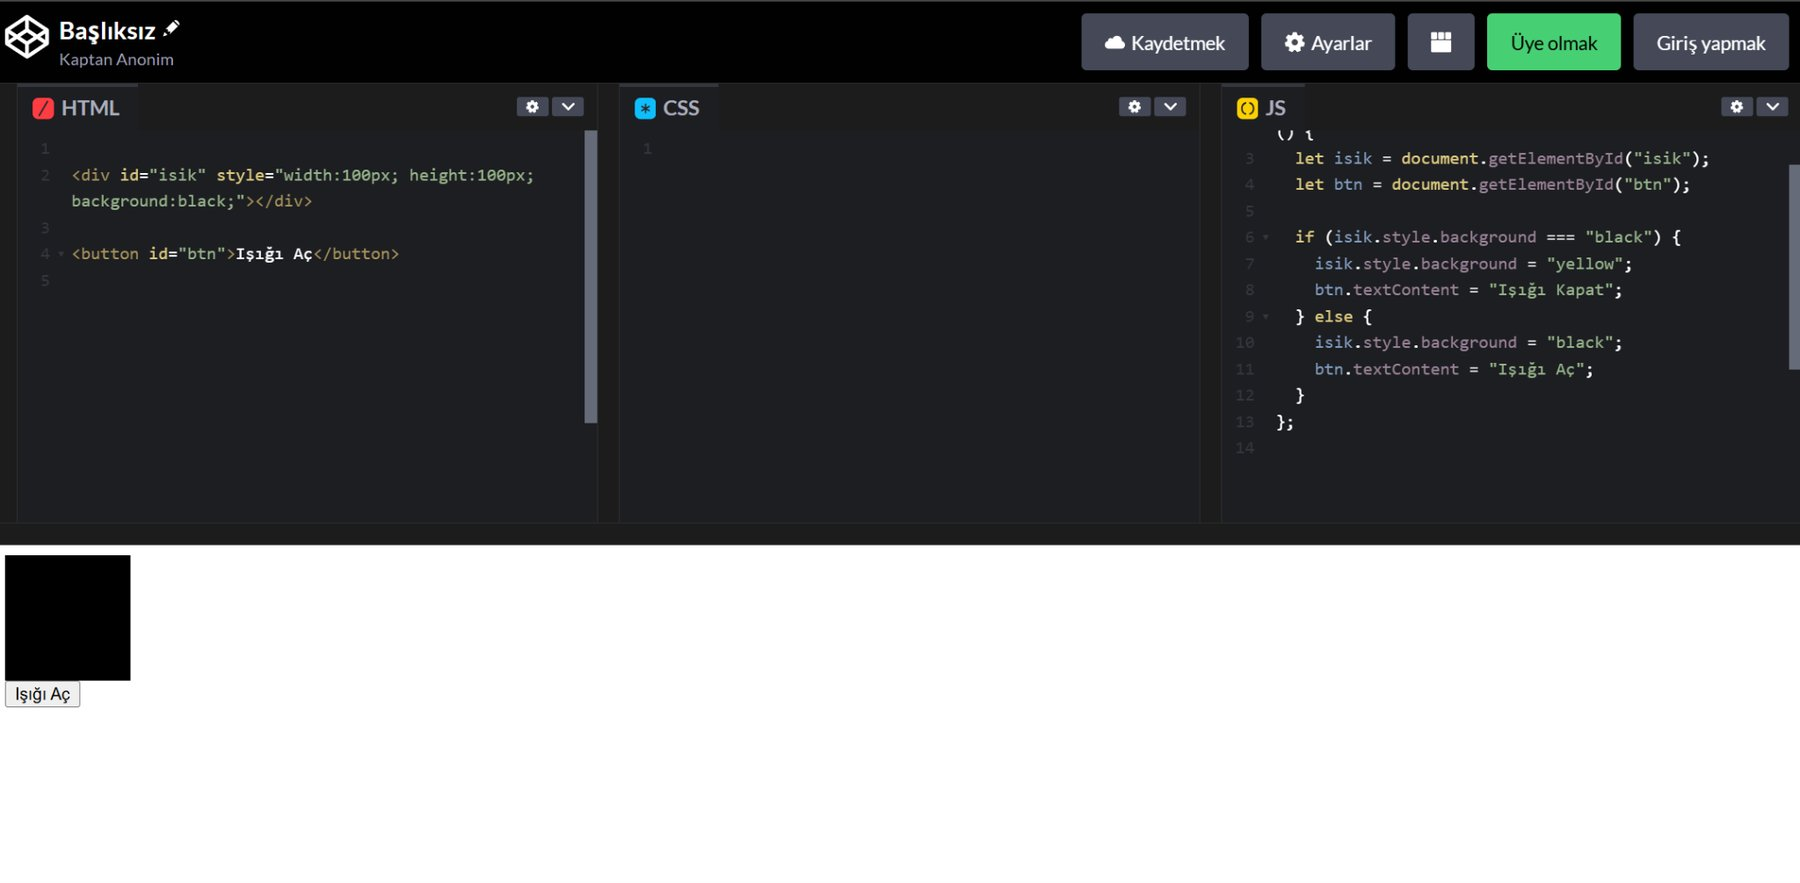
\includegraphics[width=.48\linewidth]{hafta6b.jpg}\hfill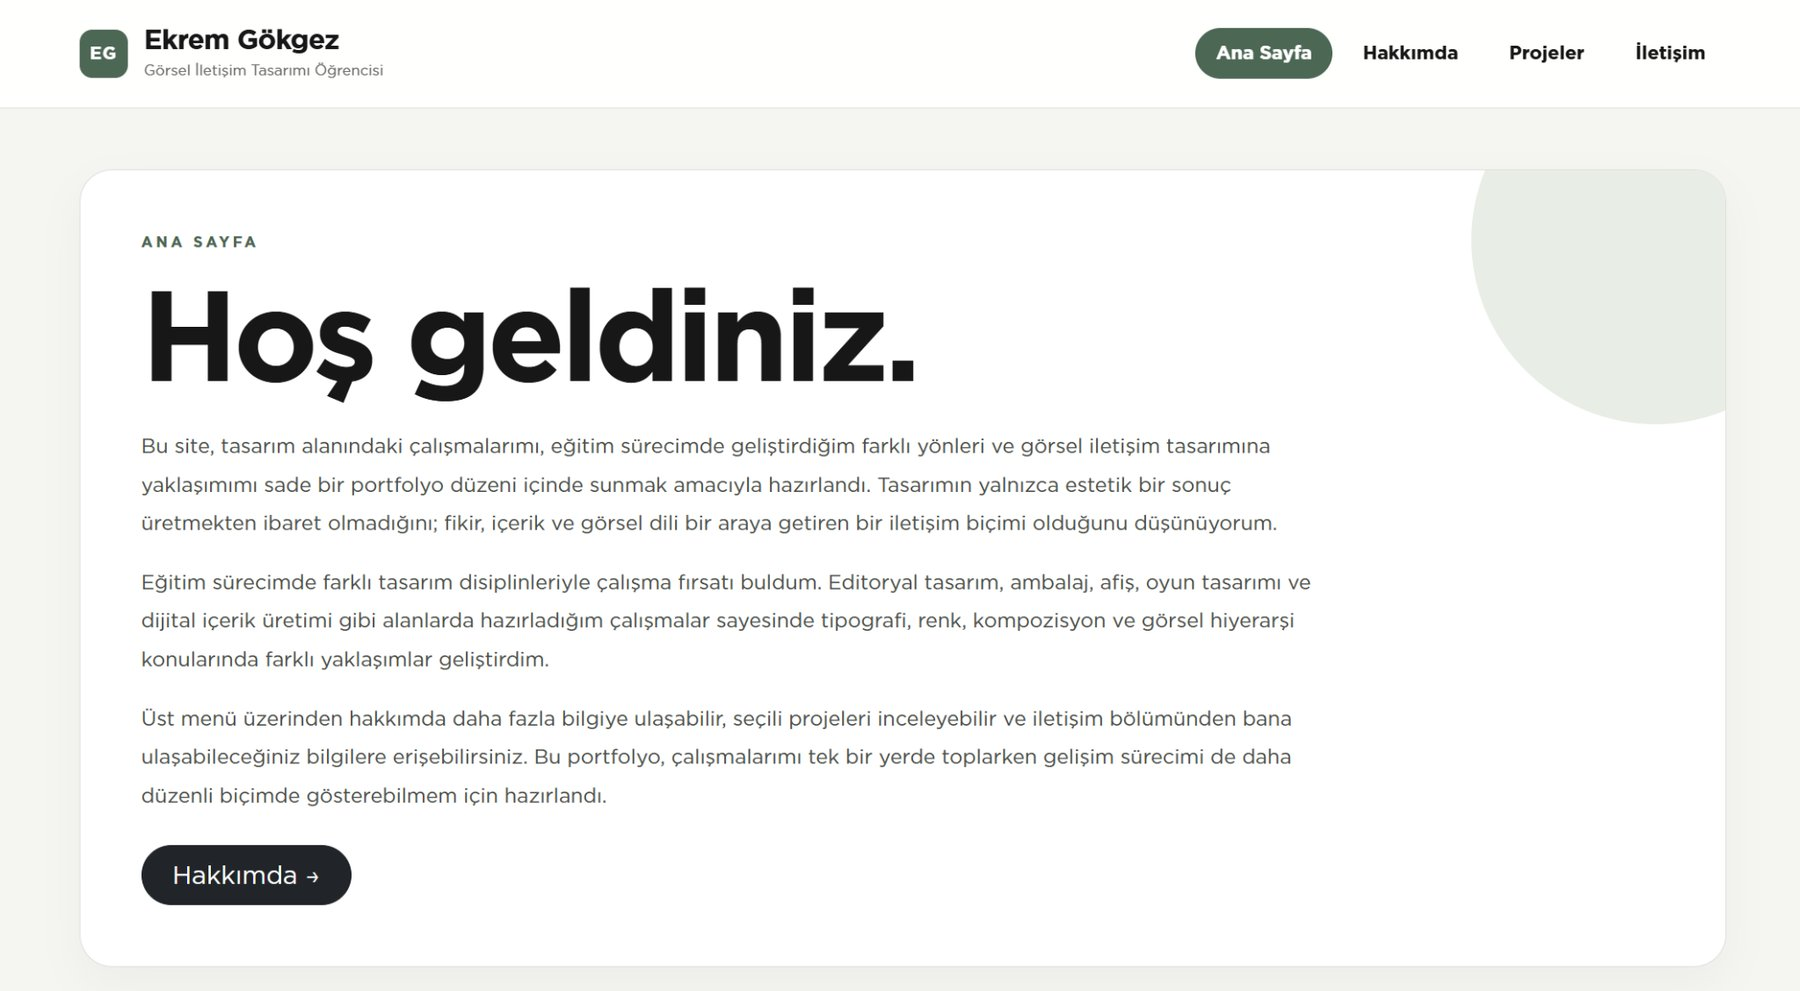
\includegraphics[width=.48\linewidth]{hafta6c.jpg}
\caption{6. hafta: JavaScript ile ışığı aç/kapat uygulaması ve portfolyo ana sayfası.}
\end{figure}
\begin{figure}[H]\centering
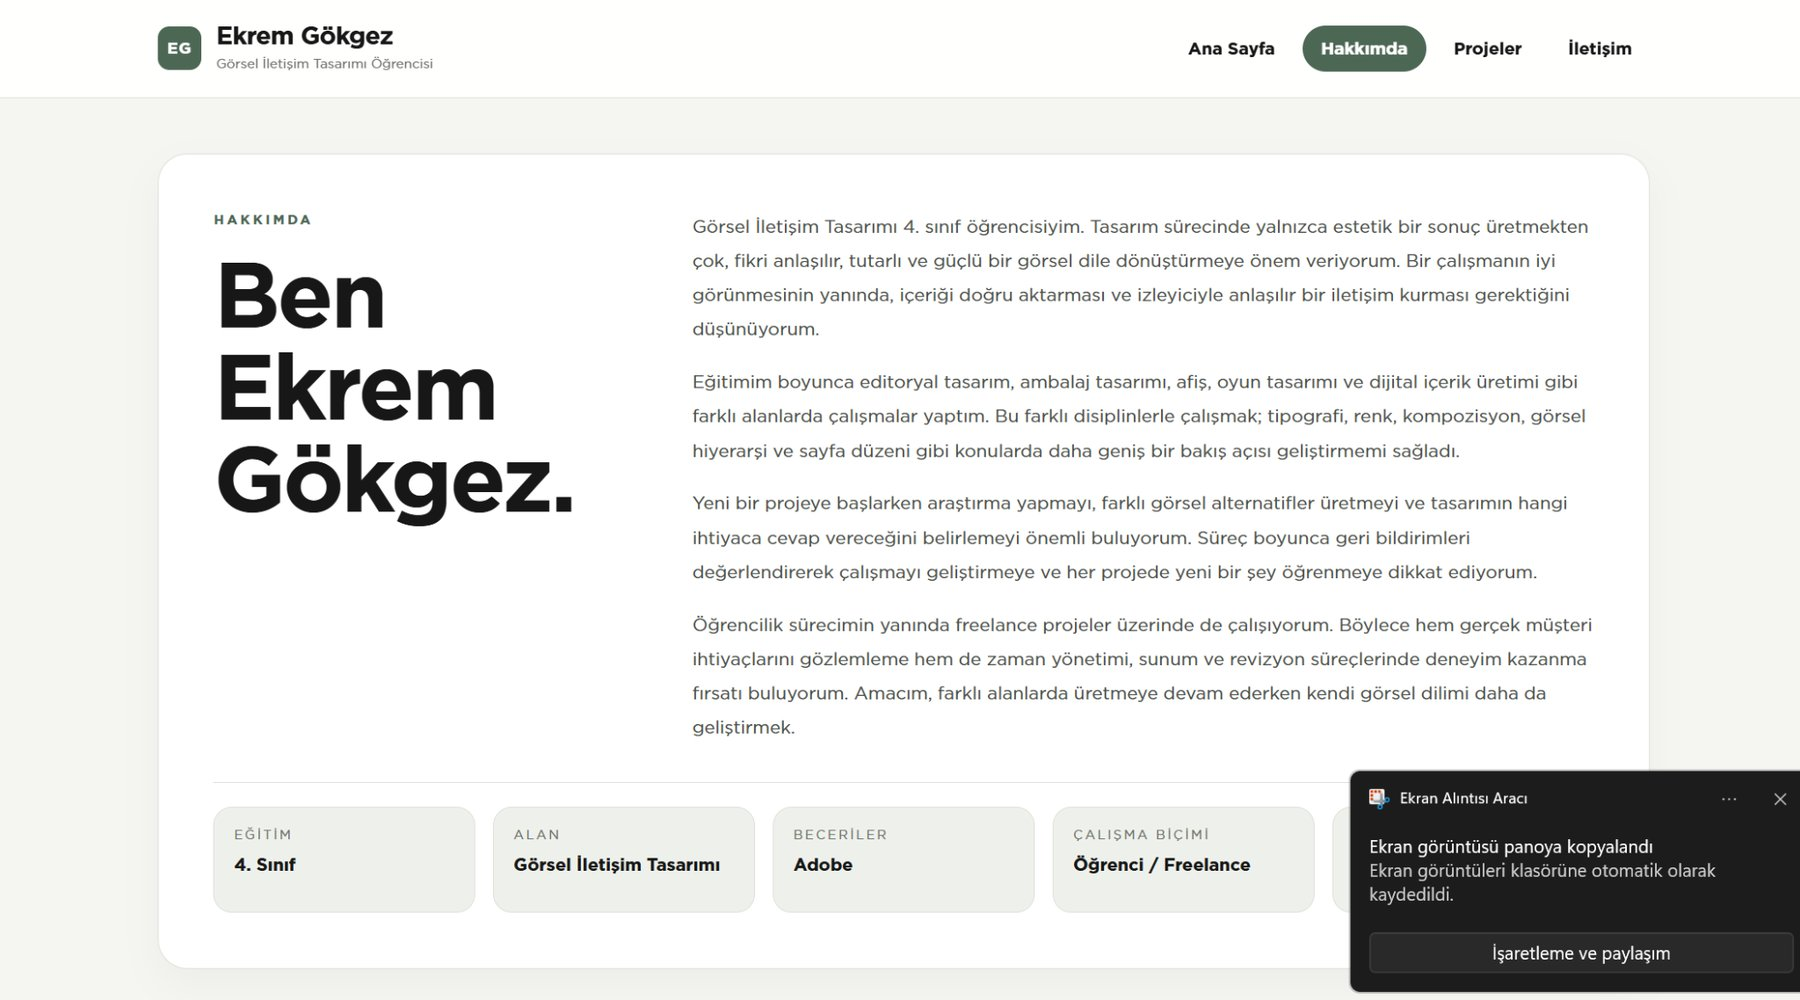
\includegraphics[width=.48\linewidth]{hafta6d.jpg}\hfill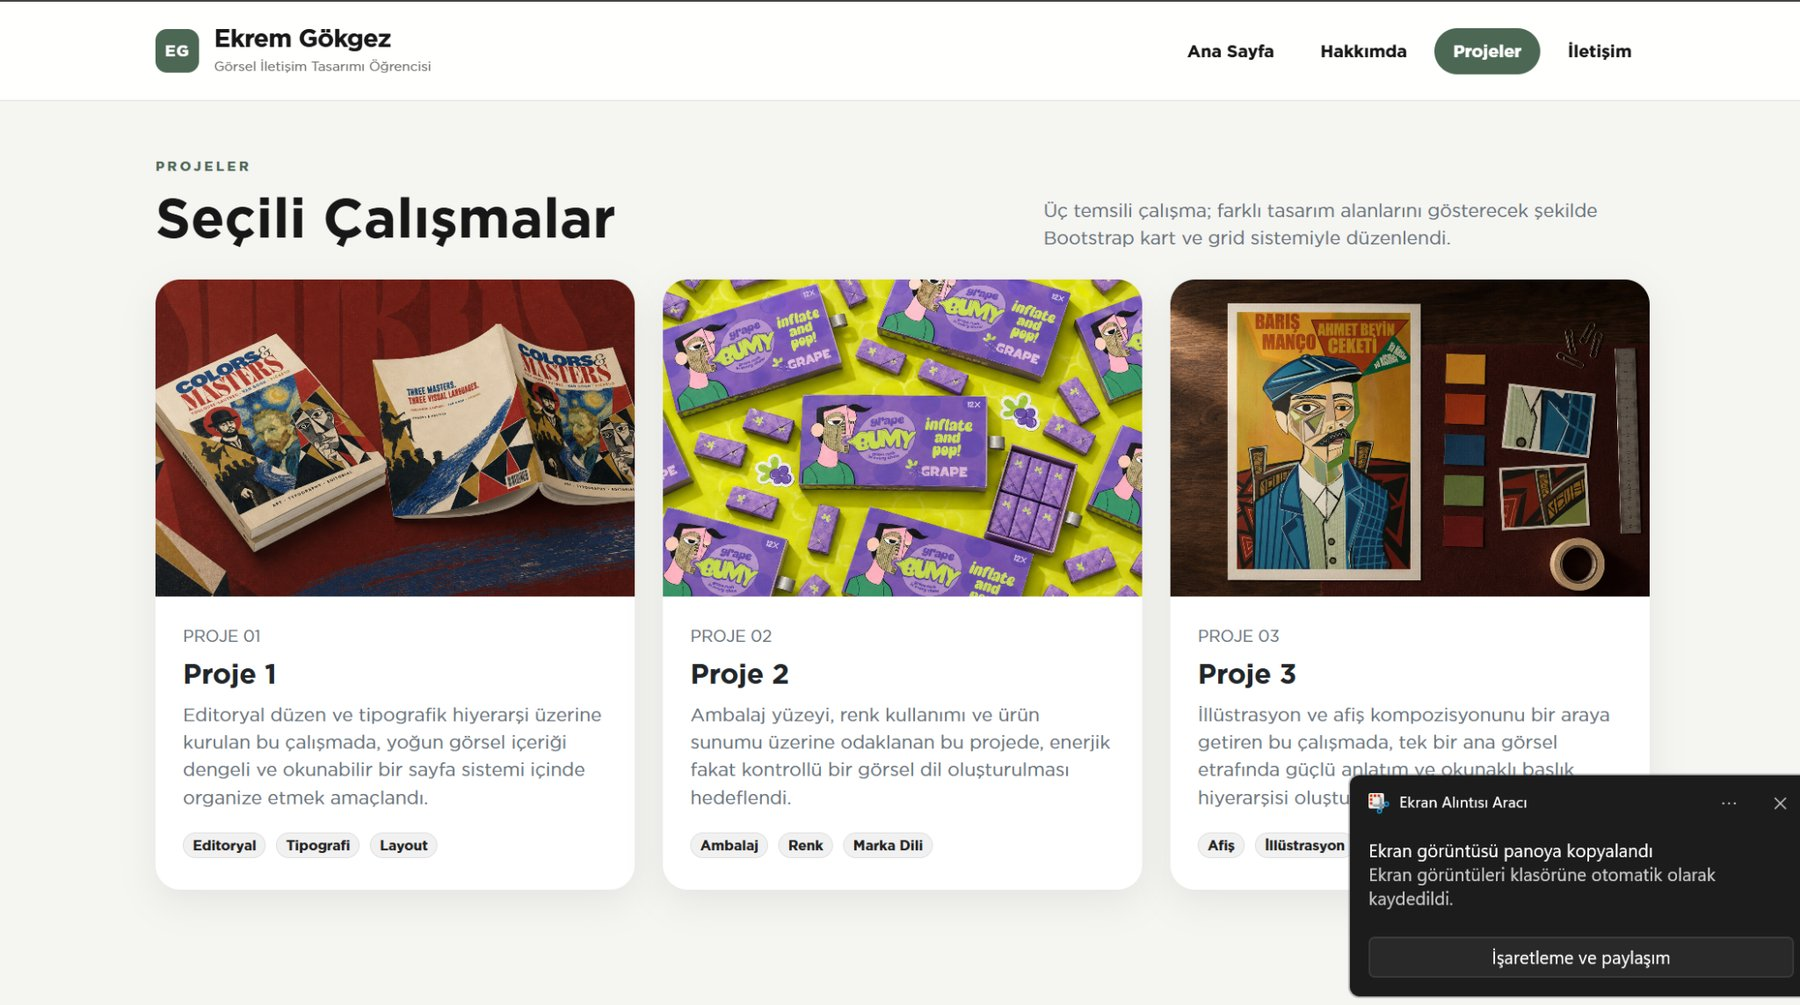
\includegraphics[width=.48\linewidth]{hafta6e.jpg}
\caption{6. hafta: portfolyonun Hakkımda ve Projeler sayfaları.}
\end{figure}
\begin{figure}[H]\centering
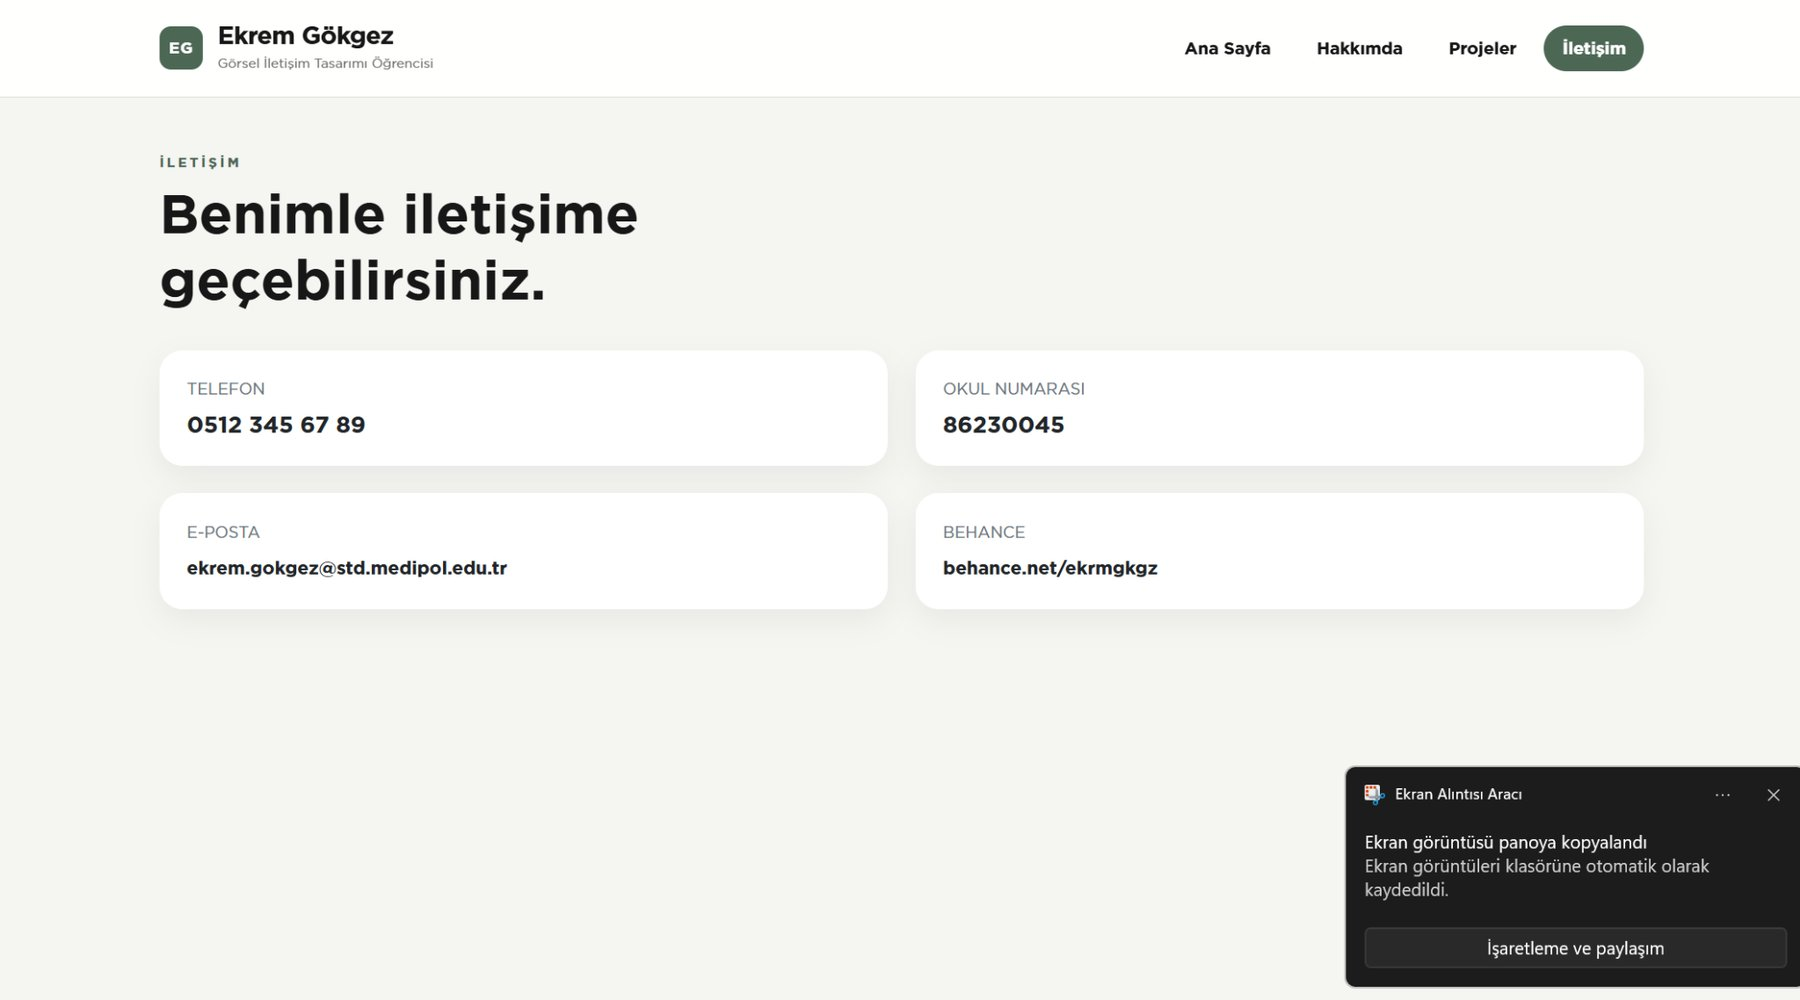
\includegraphics[width=.7\linewidth]{hafta6f.jpg}
\caption{6. hafta: kişisel portfolyonun İletişim sayfası.}
\end{figure}

\section{Test ve Değerlendirme}
MASALTI'yı bilgisayarda ve telefonda kontrol ettim. HTML dosyasını telefonun yerel önizlemesinde açtığımda bazı JavaScript özellikleri görünmedi; daha sonra GitHub Pages üzerinden açıldığında masal gezintisi, butonlar ve kaydetme işlevlerinin çalıştığını gördüm. Sayfa yenilendiğinde kaydedilen ve okunmuş masalların durumunu da kontrol ettim. Testler manuel yapılmıştır; bütün tarayıcı ve cihazlarda otomatik test uygulandığı iddia edilmemektedir.
\begin{center}
\rowcolors{2}{acik}{white}
\begin{tabular}{@{}p{5.7cm}p{3.8cm}p{3.8cm}@{}}
\toprule
\rowcolor{ana}\textcolor{white}{\textbf{Özellik}} & \textcolor{white}{\textbf{Bilgisayar}} & \textcolor{white}{\textbf{Telefon}} \\
\midrule
Masal kartları ve okuma ekranı & Görüntülendi & Mobil görünüm denendi \\
Arama, filtreleme ve gezinme & Temel işlevler denendi & GitHub Pages'te denendi \\
Kaydetme ve okundu durumu & Yeniden açınca korundu & Aynı tarayıcıda denendi \\
Yerel HTML önizlemesi & Açılıyor & Bazı JS araçları görünmedi \\
\bottomrule
\end{tabular}
\end{center}
\textbf{Denenen ortamlar:} Windows bilgisayarında tarayıcı, iPhone'da yerel HTML önizlemesi ve GitHub Pages üzerinden web tarayıcısı.\par
\textbf{GitHub:} \url{https://github.com/kseisi26-dotcom/Masalti}. Son teslim aşamasında depo içindeki HTML dosyasının adı ve bağlantıları ayrıca kontrol edilmelidir.

\section{Sunum Videosu}
Sunum videosunda proje fikrini, masalların seçimini, tasarım kararlarımı, çalışan web sitesini ve HTML/CSS/JavaScript'in temel çalışma mantığını anlatıyorum. Video kaydı alınmıştır. Raporun hazırlandığı anda YouTube yüklemesi henüz tamamlanmadığı için bağlantı ve kesin süre doğrulanamamıştır.
\begin{center}
\begin{tabular}{@{}p{4.2cm}p{9.2cm}@{}}
\textbf{Video süresi:} & Yükleme sonrası doğrulanacak (yönerge: 12--18 dakika). \\
\textbf{Görünürlük:} & Listelenmemiş veya herkese açık olarak ayarlanacak. \\
\textbf{Bağlantı:} & \youtubelink \\
\end{tabular}
\end{center}

\subsection{Video Kontrol Listesi}
\begin{itemize}[label={}]
\item $\boxtimes$ MASALTI proje, tasarım ve kod açıklaması kayda alındı.
\item $\square$ Video süresi 12--18 dakika olarak doğrulandı.
\item $\square$ Video boyunca kamera ve sesin göründüğü/duyulduğu baştan sona kontrol edildi.
\item $\square$ YouTube bağlantısı eklendi, gizli pencerede oynadığı kontrol edildi.
\item $\square$ Video yüklenmesi ve işlenmesi tamamlandı.
\item $\square$ Kapaktaki bağlantı ile bu bölümdeki bağlantı karşılaştırıldı.
\end{itemize}

\section{Sonuç ve Kendi Değerlendirmem}
Bu projede Türk masallarını görseller ve etkileşimli işlevlerle sunan bir web sitesi hazırladım. MASALTI'da öğrendiğim HTML, CSS ve JavaScript konularını daha kapsamlı bir çalışmada bir araya getirme fırsatı buldum. Görsel İletişim Tasarımı öğrencisi olarak özellikle sayfa düzenini, illüstrasyonların metinlerle ilişkisini ve tipografik hiyerarşiyi önemsedim. Kodlama sırasında yapay zekâ desteğinden yararlandım ve arayüzün ihtiyaçları doğrultusunda farklı düzenlemeler yaptım. Özellikle telefon önizlemesindeki sorun, bir dosyanın her ortamda aynı şekilde davranmayabileceğini gösterdi. GitHub Pages'te test ederek çalışan sürümü kontrol ettim. İleride daha fazla masal eklemek, okuma deneyimini erişilebilirlik açısından geliştirmek ve kullanıcı testleri yapmak isterim. Bu çalışma, bir tasarım fikrinin yalnızca görünüşten ibaret olmadığını; işlemesi ve kullanıcıya karşılık vermesi gerektiğini anlamama yardımcı oldu.

\section{Kaynakça}
Masal metinlerinin dayandığı kaynaklara sayfa içindeki ``Bu Masalın İzi'' bölümlerinden ulaşılabilir. Aşağıdaki bağlantılar projede belirtilen masal kaynaklarıdır; teknik belgeler ise HTML/CSS/JavaScript açıklamalarında yararlanılabilecek başvuru kaynaklarıdır.
{\small
\begin{thebibliography}{15}
\bibitem{ok1} Okuryazar. \emph{Ali Cengiz Oyunu}. \url{https://www.okuryazar.com.tr/dergi/ali-cengiz-oyunu}.
\bibitem{ok2} Okuryazar. \emph{Balıkçının Oğlu}. \url{https://www.okuryazar.com.tr/dergi/balikcinin-oglu}.
\bibitem{ok3} Okuryazar. \emph{Değirmenci ile Tilki}. \url{https://www.okuryazar.com.tr/dergi/degirmenci-ile-tilki}.
\bibitem{kp1} Kültür Portalı. \emph{Dört Öğüt}. \url{https://www.kulturportali.gov.tr/portal/dortogut-1}.
\bibitem{kp2} Kültür Portalı. \emph{Kabak Gelin}. \url{https://www.kulturportali.gov.tr/portal/kabakgelin}.
\bibitem{kp3} Kültür Portalı. \emph{Keloğlan ile Yılan, Köpek, Kedi ve Balık}. \url{https://www.kulturportali.gov.tr/portal/keloglanileyilankopekkedivebalik}.
\bibitem{kp4} Kültür Portalı. \emph{Keloğlan ve Altın Bülbül Masalı}. \url{https://www.kulturportali.gov.tr/portal/keloglanvealtinbulbulmasali}.
\bibitem{kp5} Kültür Portalı. \emph{Korkak Adam ve Devler}. \url{https://www.kulturportali.gov.tr/portal/korkakadamvedevler}.
\bibitem{md1} Masal Dergisi. \emph{Tuz Kadar Sevgi}, sayı 28 (2025). \url{https://www.masaldergisi.com/sayilar/2025/sayi-28/tuz-kadar-sevgi/}.
\bibitem{ok4} Okuryazar. \emph{Üç Turunçlar}. \url{https://www.okuryazar.com.tr/dergi/uc-turunclar}.
\bibitem{mdnhtml} MDN Web Docs. \emph{HTML elements reference}. \url{https://developer.mozilla.org/en-US/docs/Web/HTML/Reference/Elements}.
\bibitem{mdncss} MDN Web Docs. \emph{CSS media queries}. \url{https://developer.mozilla.org/en-US/docs/Web/CSS/Guides/Media_queries}.
\bibitem{mdnjs} MDN Web Docs. \emph{Window: localStorage property}. \url{https://developer.mozilla.org/en-US/docs/Web/API/Window/localStorage}.
\end{thebibliography}}

\appendix
\section{Teslim Kontrol Listesi}
\begin{itemize}[label={}]
\item $\square$ MEBİS'e yalnızca rapor PDF'i yüklendi.
\item $\boxtimes$ PDF adı \texttt{86230045\_EkremGokgez\_vize.pdf} biçiminde düzenlendi.
\item $\square$ GitHub ve YouTube bağlantıları son kez kontrol edildi.
\item $\square$ GitHub deposuna son rapor PDF'i, \texttt{main.tex} ve görseller yüklendi.
\item $\boxtimes$ GitHub deposu herkese açık olarak oluşturuldu.
\item $\square$ Teslim saatinden önceki son commit ve dosya düzeni doğrulandı.
\item $\boxtimes$ Proje tek HTML dosyasında içsel CSS ve JavaScript içeriyor.
\item $\boxtimes$ Yapay zekâ kullanımı raporda açıklandı.
\item $\boxtimes$ Web sitesinin temel işlevleri ve kod yapısı sunumda anlatıldı.
\end{itemize}
\textbf{Teslim öncesi eksikler:} YouTube bağlantısı, video süresinin doğrulanması ve raporun GitHub'a yüklenip MEBİS'e teslim edilmesidir. Bu satır, son kontroller tamamlanınca güncellenebilir.

\end{document}
